\documentclass[12pt]{article}

\usepackage{amsthm}
\usepackage{amsmath}
\usepackage{amsfonts}
\usepackage{graphicx}
\usepackage{hyperref}
\usepackage{algorithm}
\usepackage{algpseudocode}
\usepackage{subcaption}
\usepackage{caption}
\usepackage{wrapfig}
\usepackage{cite}

\newcommand{\fft}{\text{FFT}}
\newcommand{\ifft}{\text{IFFT}}

\title{Audio Transport}
\date{\today}
\author{Trevor Henderson}

\begin{document}
\maketitle

\begin{abstract}
  This paper describes a new technique to interpolate between audio signals.
  This technique uses optimal transport to move the pitches in one signal to the pitches in another.
  Audibly this sounds like a generalized portamento, or glide between sounds.
  The main contributions of this paper are methods to remove the different types of phasing distortion that can occur in a naive transport.
  A real time implementation of the algorithm produces musical results.
  \\
  \\
  Code: \href{https://github.com/sportdeath/Vocoder}{https://github.com/sportdeath/Vocoder}.
  \\
  Video: \href{https://youtu.be/PQGV0fk3Gww}{https://youtu.be/PQGV0fk3Gww}
\end{abstract}

\section{Introduction}

A portamento is a musical term used to describe one pitch sliding into another.
The portamento can be found in almost all genres of music, 
whether it is a slur in a vocal passage or in the twang of a slide guitar.
It provides smooth way to transition between notes and even chords.

This effect, though widely used, is limited in its use by the physical design of the instrument. 
Most acoustic keyboard instruments for example, like the piano or organ, can't glide at all because notes are formed from a discrete set of strings or pipes. 
Digital keyboards can produce a glide with  a pitch wheel.
The pitch wheel can change the playback rate of a sample as it plays or use spectral time stretching to change the pitch of a prerecorded audio sample.
However, this system does not make it easy to slide between chords of different shapes.
And moreover, it is impossible to slide between sounds with different timbres.

This paper describes a method to produce a portamento not only between sounds with different timbres but between sounds from different instruments entirely.
It does this using optimal transport, a geometric technique typically found in applications to computer graphics and machine learning.

The optimal transport problem seeks a map between two probability masses in $\mathbb{R}^n$ that minimizes the work done on the mass.
Mass in the transport must physically move through space and all mass must be preserved.
\begin{figure}
  %{r}{0.65\textwidth}
  \begin{center}
  \begin{subfigure}[b]{0.45\textwidth}
    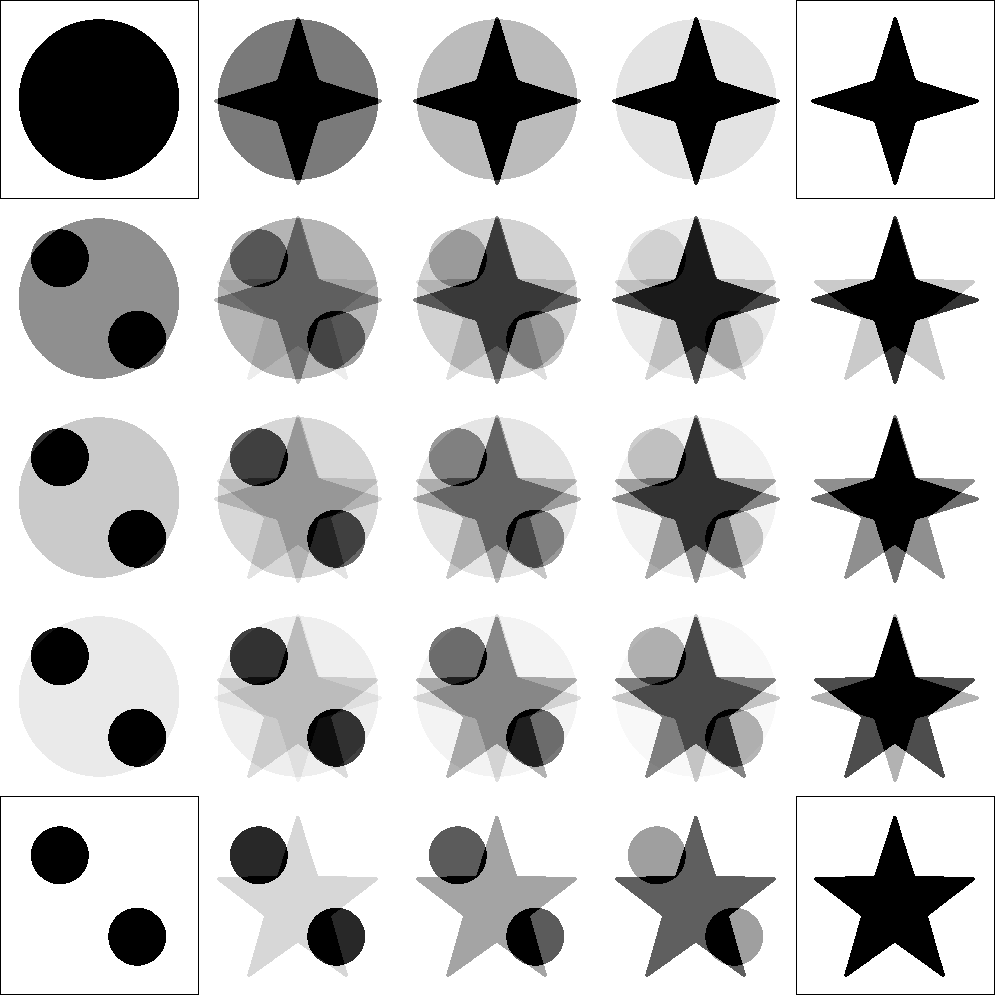
\includegraphics[trim={0 27.5cm 0 0},clip,width=\textwidth]{figures/euclidean_gray}
    \caption{Linear Interpolation}
    \label{fig:linear}
  \end{subfigure}
  \hspace{1cm}
  \begin{subfigure}[b]{0.45\textwidth}
    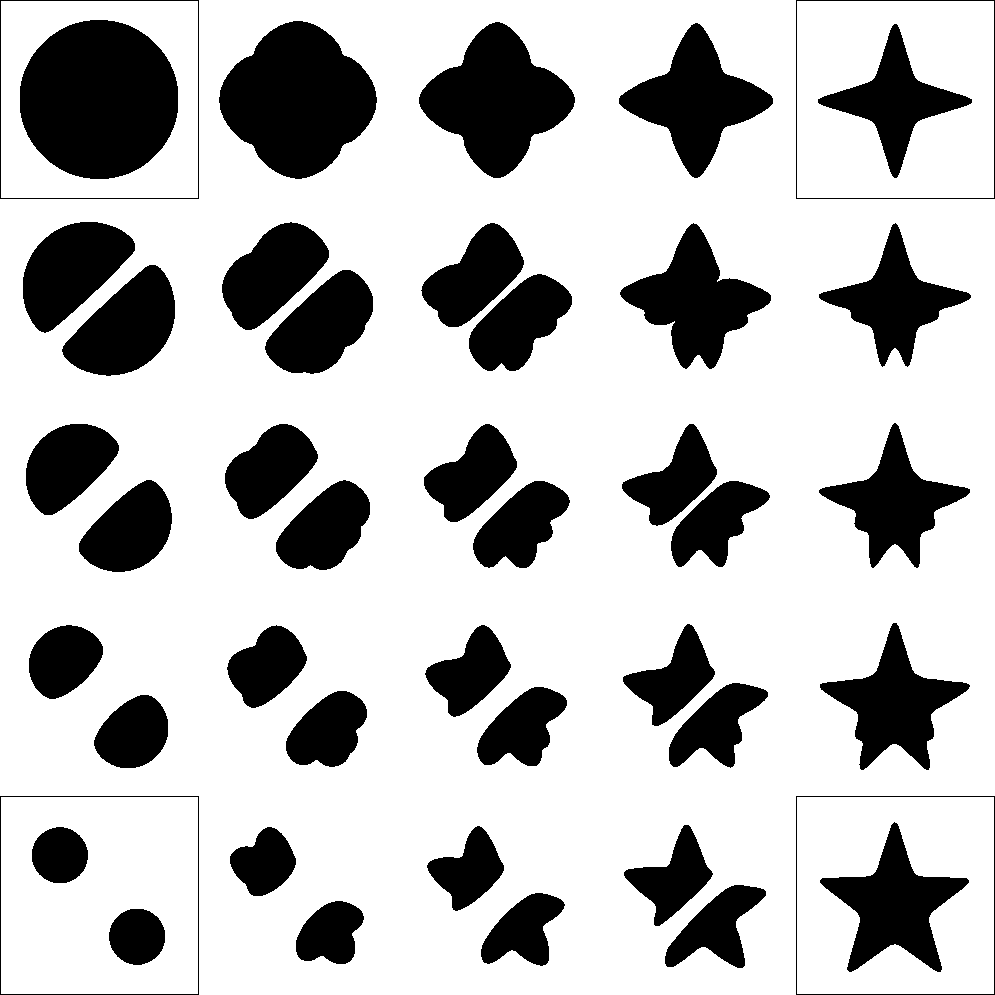
\includegraphics[trim={0 27.5cm 0 0},clip,width=\textwidth]{figures/wasserstein}
    \caption{Optimal Transport Interpolation}
    \label{fig:wasserstein}
  \end{subfigure}
  \end{center}
  \caption{From \emph{Convolutional Wasserstien Distances: Efficient Optimal Transportation on Geometric Domains} by Justin Solomon et al, 2015\cite{justin}}
  \label{fig:justin}
\end{figure}
I find that optimal transport is best explained visually as in figure~\ref{fig:justin} from Justin Solomon et al \cite{justin}.
Efficient solutions to compute an optimal transport mapping is an open problem 
for $n > 1$.
However, optimal transport on the real line has a closed form solution.

We will use optimal transport on the real line to find a mapping between the spectra of two audio sources that minimizes the distances that the pitches move. 
From this assumption we can guarantee that no pitches will cross each other.

\section{Contributions}

I developed a new technique to interpolate between two audio signals using optimal transport.
The optimal transport problem is usually only defined only for positive real inputs. 
The spectra of an audio signal however is complex.
It is natural that the transport be done on the absolute values of these complex numbers, but this begs the question of what is to be done with the phase.

This paper describes several types of distortion that can occur because of phasing issues and how to resolve them. 
These problems are similar to those experienced in phase vocoders --- the technology that allows an audio signal's speed to be changed without changing the pitch.
However the solutions posed in this paper improve upon the techniques used in phase vocoders and take advantage of the specifics of this problem set up.
\cite{vocoder}

These are the main techniques used in the algorithm which are new to this paper:
\begin{enumerate}
  \item
    A method to segment and audio spectrum into groups whose local phase relations have audible significance.
  \item
    A method to update the phase of a pitch shifted signal given a source and destination.
\end{enumerate}

Additionally we also provide a real-time implementation of the algorithm for audible demonstration.

\section{Related Work}

Many audio tools exist that modulate the pitch of an audio signal.
The phase vocoder, also given other names in application like `time-warping,' became practical in the early 2000's, is now pervasive in all types of music production\cite{vocoder}\cite{ableton}. It is useful to piece together samples played in different keys, or to fine tune a recording.
The phase vocoder is also the technology that enables auto-tune --- an effect which swept through the music industry in the mid-2000's and is still popular today.

Several audio tools work to manipulate the pitches within an audio signal separately.
Melodyne is a popular tool in the music industry for correcting the pitches of notes.
In 2008, Melodyne released a feature to adjust the pitches of individual notes in polyphonic music, allowing a user to rewrite the harmony of a song
\cite{melodyne}.
This technology works on a static audio file, but in 2012 a product named Zynaptiq allows for different bands of an audio stream to be pitch shifted
\cite{zynaptiq}.

However neither of these products pitch shift on with granularity that is needed to slide between notes of different timbres.
In addition, they rely on the user to select which notes they would like to tune.
While this is an extremely useful feature in the studio, it is hard to control in the live setting. 

Optimal transport has been used for audio processing before.
However so far as I can tell, no paper has synthesized sound with optimal transport.
Most of the existing papers in this cross section use optimal transport to help transcribe music.
Using a distance metric based on the harmonic series seems to be useful for determining fundamental of a note\cite{musictransport1}\cite{musictransport2}.

\section{Algorithm Overview}

\subsection{STFT}

Like almost all spectral algorithms, this one begins with a short-time Fourier transform (STFT) and ends with it's inverse (ISTFT).
At the cost of reduced temporal resolution, the STFT gives us access to the spectral components of the signal in time.
The following summarizes the relavant properties of the STFT for this problem as described by Julius O. Smith III in \emph{Spectral Audio Signal Processing} \cite{dsprelated}.

The STFT performs a discrete time Fourier transforms on windows of size $M$ of the original signal $x(n)$.
These windows are separated by a hop size of $R$. The $\tau$th frame of the STFT is
\begin{align}
  X(\omega, \tau) = 
  \text{DTFT}(\tilde{x}(n, \tau)w(n))
\end{align}
where
\begin{align}
  \tilde{x}(n,\tau) = x(n + \tau R)
\end{align}
is a buffer of the original signal, shifted $R$ samples from the previous buffer and $w(n)$ is the synthesis window.
$w(n)$ is defined to be nonzero for $M$ samples, 
$n\in\left[-\frac{M - 1}{2}, \frac{M - 1}{2}\right]$, so only the $M$ most recent samples of $x(n)$ need to be kept in memory.

After some computation, 
we produce frames $Y(\omega, \tau)$ 
which we want to use to synthesize the signal $y(n)$.
We perform this ISTFT using the weighted overlap add method.
As the name suggests, this method works by
overlapping adjacent frames of the IDTFT, 
weighting them by an analysis window $f(n)$ 
and then adding them together.
The weighting helps to suppress audible discontinuities at frame boundaries
which prevents artifacts in highly nonlinear filters such as the one this paper describes.
\begin{align}
  \tilde{y}(n,\tau) &= \text{IDTFT}(Y(\omega, \tau))
  \\
  y(n) &= \sum_\tau f(n - \tau R)\tilde{y}(n - \tau R,\tau)
\end{align}
Note that synthesizing a single sample of $y(n)$ requires overlapping
$\frac{M}{R}$ frames which adds a latency of $M$ samples between $y$ and it's sources.

In the absence of spectral modifications, 
we can achieve perfect reconstruction 
of a signal transformed by the STFT and ISTFT given
that the synthesis and analysis windows obey
\begin{align}
  \sum_\tau w(n - \tau R)f(n - \tau R) = 1,\; \forall n\in \mathbb{Z}
\end{align}
I chose to use the square root of the Hann window as both the analysis and frequency window
which gives perfect reconstruction when $R = \frac{M}{2k}$ for $k\in\mathbb{Z}$.
\begin{align}
  w(n) = 
  f(n) =
  \cos(\pi n / M)
  %, 
  %n\in
  %\left[
  %-\frac{M-1}{2}, 
  %\frac{M-1}{2}
%\right]
\end{align}

For actual computation we replace, the DTFT and IDTFT with the FFT and IFFT respectively. 
The FFT has $M$ bins $n\in\left[-\frac{M - 1}{2}, \frac{M - 1}{2}\right]$.
The frequency of the $n$th bin is given by
\begin{align}
  \omega = 2\pi\frac{f_s n}{M}
\end{align}
where $f_s$ is sampling rate of the signal.
Since the audio signal $x(n)$ is real, $X(\omega)$ is conjugate symmetric, so we only need to retain the positive bins $\left[0, \frac{M - 1}{2}\right]$ of the FFT.

\subsection{Spectrum Segmentation}

\begin{figure}[!h]
  %{r}{0.65\textwidth}
  \begin{center}
  \begin{subfigure}[b]{0.65\textwidth}
    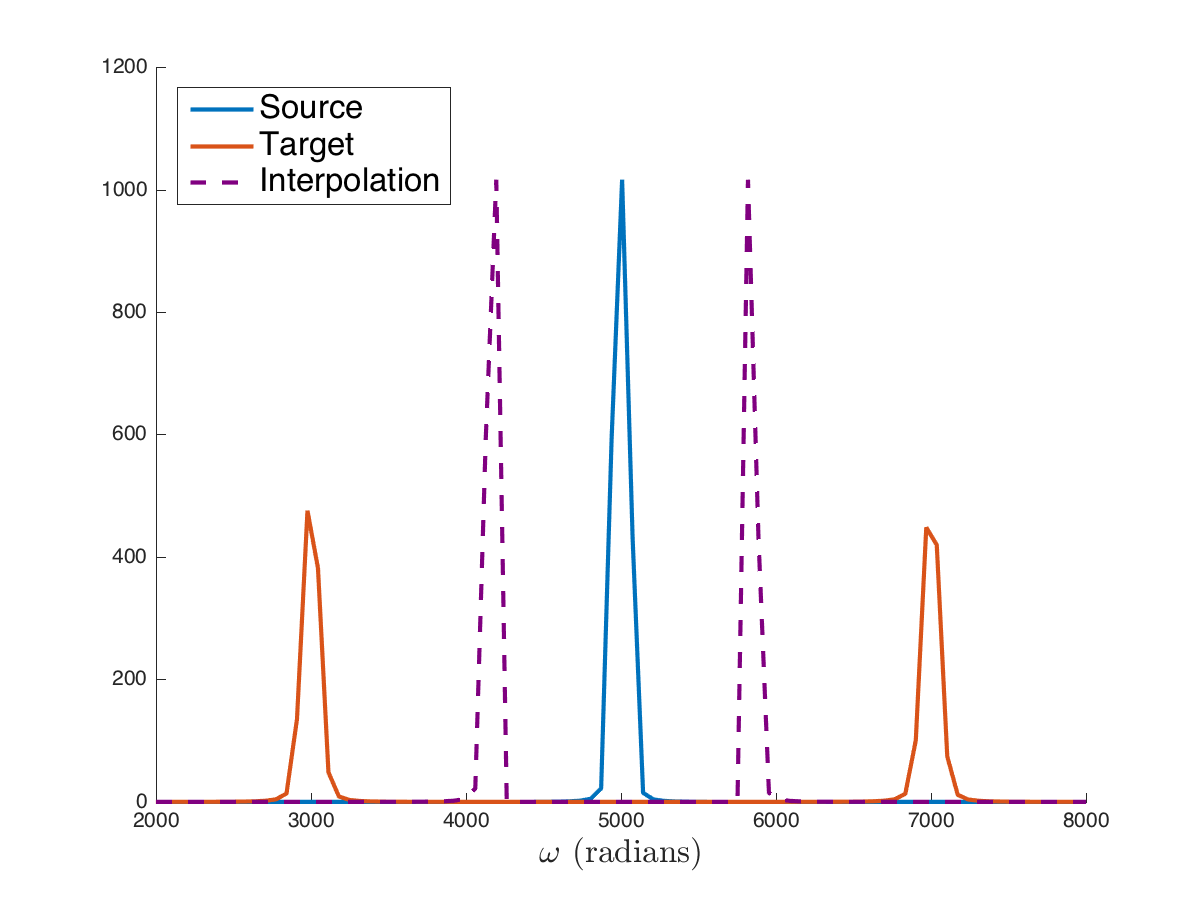
\includegraphics[width=\textwidth]{figures/VerticalIncoherence0}
    \caption{Interpolated Spectra}
    \label{fig:verticalincoherence0}
  \end{subfigure}
  \hspace{1cm}
  \begin{subfigure}[b]{0.65\textwidth}
    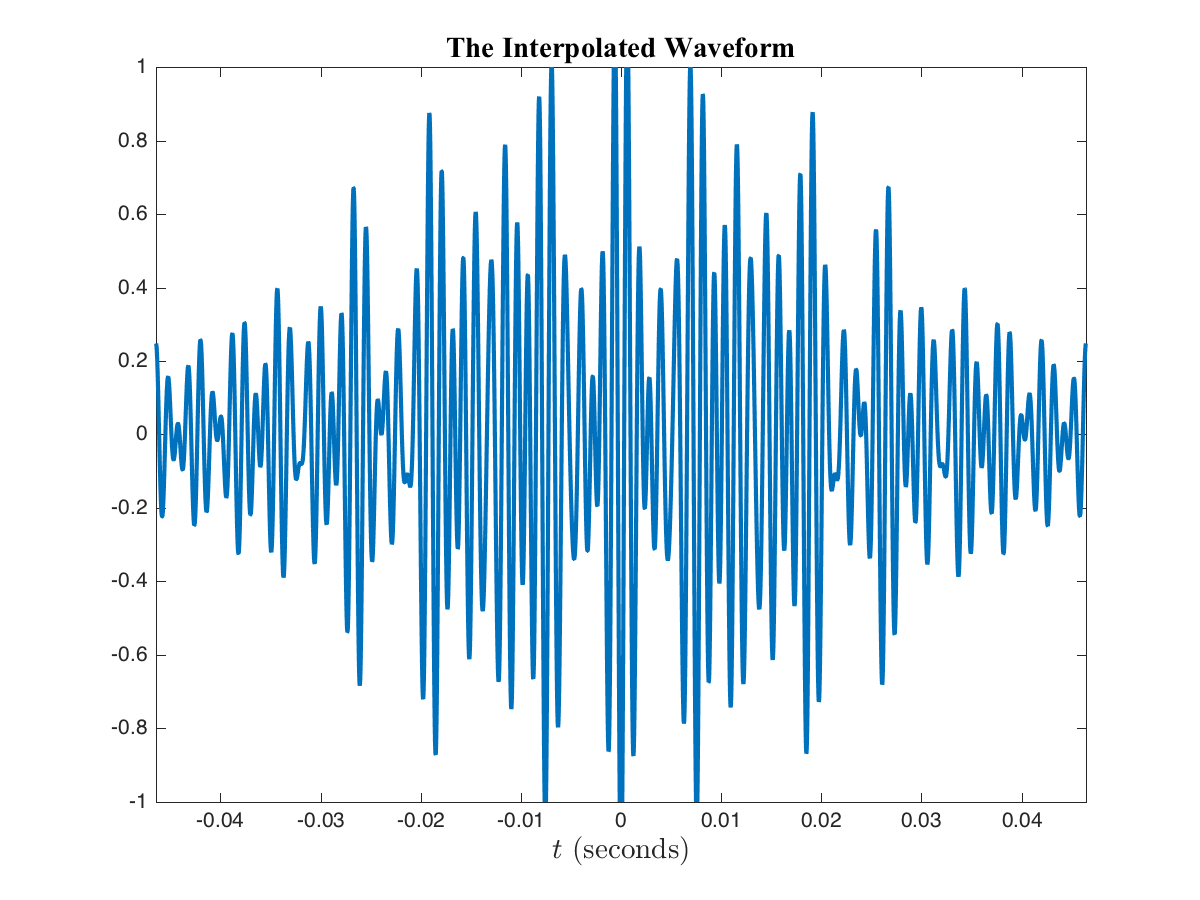
\includegraphics[width=\textwidth]{figures/VerticalIncoherence1}
    \caption{Interpolated Waveform}
    \label{fig:verticalincoherence1}
  \end{subfigure}
  \end{center}
  \caption{%
    If we perform a transport across all bins,
    sinusoids smeared across multiple bins can be split in two (\ref{fig:verticalincoherence0}).
    The resulting waveform 
    (\ref{fig:verticalincoherence1}) should the sum of two sinusoids, but it
    experiences distortion
    known as \emph{vertical incoherence}.
    %If we do optimal transport on the amplitudes, we end up splitting the .
    %The lower plot is the interpolation of sinusoids using this method.
    %It is obviously distorted with what is known as \emph{vertical incoherence} --- phasing distortion within a window of the STFT.
  }
  \label{fig:verticalincoherence}
\end{figure}

Once we have the spectrum $X_0$ from one window of the STFT, we then want to transport it to another spectrum $X_1$ from a separate STFT running in parallel.
However performing a transport across all bins results in distortion as seen in figure~\ref{fig:verticalincoherence}.
This distortion is known as vertical incoherence in phase vocoder algorithms. It occurs when local phase relations pertaining to a particular frequency component are lost
\cite{vocoder}.

A technique that is used to fix this problem in phase vocoders is to lock the phases of particular regions of the spectrum
\cite{vocoder}.
For this problem, this means we must do the transport on chunks of the spectrum rather than the individual bins.
All that is needed now is an algorithm to segment the spectrum into pieces whose phase relations we want to maintain.

Phase vocoder algorithms often use peak finding to determine these regions
\cite{vocoder}.
However, peak finding is not very robust to noise. 
Any small oscillation in the transform 
can cause an unnecessary split and produce vertical incoherence.
This does not seem to effect the performance of the phase vocoder because all of these regions are moving to the same pitch.
But the effect becomes much more noticeable when suddenly all regions are moving to entirely different pitches.
Adding a noise threshold not only makes the segmentation less elegant, it also begins to ignore high frequency components, which typically have a much smaller amplitude.

\begin{figure}[!h]
  %{r}{0.65\textwidth}
  \begin{center}
  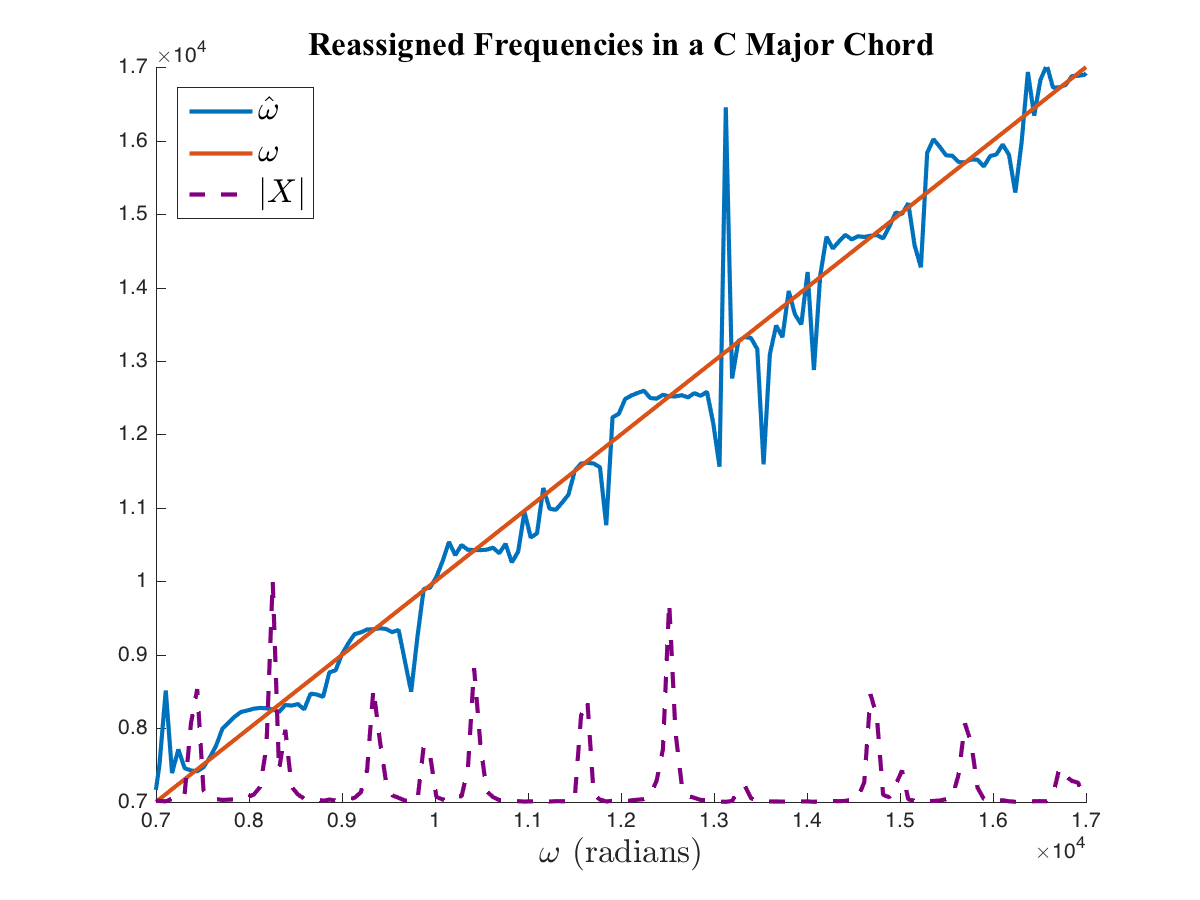
\includegraphics[width=0.7\textwidth]{figures/ReassignedFreqCMaj}
  \caption{The reassigned frequencies in a C Major chord played on the piano}
  \label{fig:reassignedfrequency}
\end{center}
\end{figure}

Instead, I determine where to split the window based on the \emph{reassigned frequency}, $\hat{\omega}(\omega)$.
The reassigned frequency as shown in figure~\ref{fig:reassignedfrequency} 
is a more accurate notion of the frequency a bin is actually oscillating at.
A sinusoid smeared over multiple bins for example, should have a constant reassigned frequency, because the smeared amplitudes all support the center frequency.
Likewise, many of the peaks in the spectrum of the piano chord in figure~\ref{fig:reassignedfrequency} align with relatively flat sections of the reassigned frequency
\cite{reassignment}.

\begin{algorithm}
  \caption{Segment Spectrum}\label{segment}
\begin{algorithmic}
  \State{$S\leftarrow\{\}$}
  \State{$s\leftarrow\emptyset$}
  \For{each bin $n>0$}
    \State{$U(s) \leftarrow U(s)\cup n$}

    \\
    \If{%
      $\hat{\omega}(n - 1) - \omega(n - 1) > 0$ and
      $\hat{\omega}(n) - \omega(n) < 0$}
      \State{// \emph{$\hat{\omega}$ crosses down through $\omega$}}
      \State{// \emph{Make a center of mass}}
      \State{$c(s) \leftarrow n - 1$}
      \\
    \ElsIf{%
      $\hat{\omega}(n - 1) - \omega(n - 1) < 0$ and
      $\hat{\omega}(n) - \omega(n) > 0$}
      \State{// \emph{$\hat{\omega}$ crosses up through $\omega$}}
      \State{// \emph{Split the mass}}
      \State{$S\leftarrow S\cup\{s\}$}
      \State{$s\leftarrow\emptyset$}
    \EndIf
  \EndFor
\end{algorithmic}
\end{algorithm}
Once the reassigned frequency has been computed, we can use algorithm~\ref{segment} to segment the spectrum into a set $S$ of spectral pieces $s(i)$.
Each piece $s$ is defined by its center of mass $c(s)$, its set of bins $U(s)$, and a mass $\rho(s)$.
The center of the mass is picked so that it is the bin whose frequency is closest to the reassigned frequency.
The mass of each segment is a normalized sum of its components
\begin{align}
  \rho(s) = \frac{\sum_{n\in U(s)}|X(n)|}{\sum_{n}|X(n)|}
\end{align}
This normalization occurs so that the sum of masses equals 1 for optimal transport:
\begin{align}
  \sum_{s\in S} \rho(s) = 1
\end{align}

\begin{figure}[!h]
  %{r}{0.65\textwidth}
  \begin{center}
  \includegraphics[width=0.7\textwidth]{figures/SegmentedReassignedFreqCMaj}
  \caption{The segmentation produced by algorithm~\ref{segment}. Centers of mass are marked in green and the boundaries between masses are marked in black.}
  \label{fig:segmentation}
\end{center}
\end{figure}

Figure~\ref{fig:segmentation} shows a segmentation performed by the algorithm.
The figure shows that many of the center of mass marked in green align exactly with the peak. 
However the small peak near $\omega = 8000 \;\text{radians}\cdot \text{s}^{-1}$ is ignored because it is dominated by the larger peak next to it which still exerts influence.

\begin{figure}[!h]
  %{r}{0.65\textwidth}
  \begin{center}
  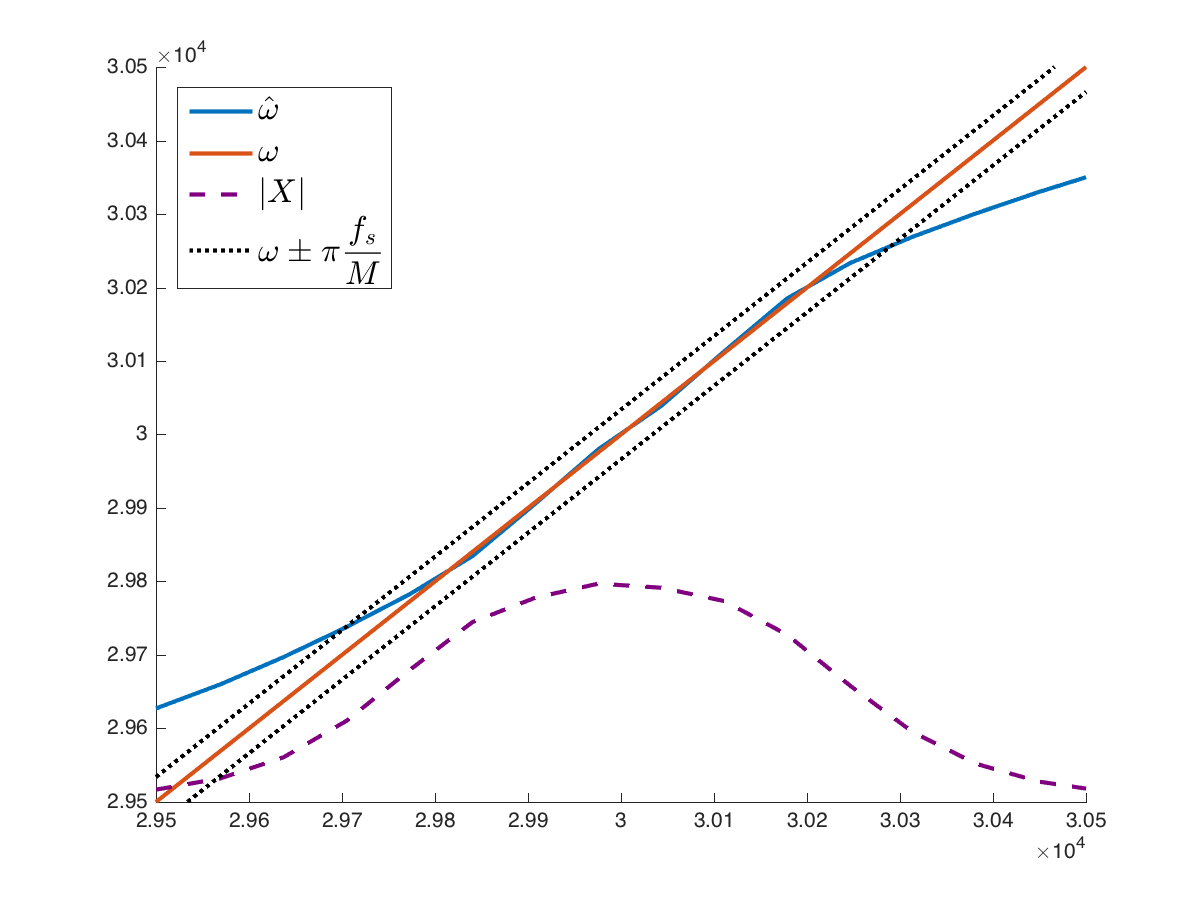
\includegraphics[width=0.7\textwidth]{figures/ReassignedFreqChri1}
  \caption{The reassigned frequency of a linear chirp --- a sinusoid with linearly increasing amplitude. The reassigned frequency is approximately linear over the chirps range. The dotted black lines show a region where small fluctuations do not produce new segmentations.}
    \label{fig:chirp}
  \end{center}
\end{figure}

A slight modification must be made to this algorithm to account for audio where the relation between frequency and reassigned frequency is relatively linear as shown in figure~\ref{fig:chirp}. In these cases, slight perturbations in the reassigned frequency with cause it to fluctuate over and under the bin frequency producing unnecessary segmentations.
We resolve this by adding a boundary region whose width is equal to the width of an FFT bin, $2\pi \frac{f_s}{M}$.
The algorithm is essentially the same only we form masses when we cross up through the entire boundary region
and define our center of masses when we cross down through the entire boundary region.

The reassigned frequency can be computed as follows \cite{reassignment}:
\begin{align}
  \hat{\omega}(\omega) = 
  \omega + 
  \Im\left\{%
    \frac{X_\mathcal{D}(\omega)\cdot X^*(\omega)}{|X(\omega)|^2}
  \right\}
\end{align}
where $X_\mathcal{D}$ is the spectrum of the input signal $x(n)$ windowed with
$w_\mathcal{D}(n) = \frac{d}{dt}w(n)$:
\begin{align}
  X_\mathcal{D}(\omega) = \fft\left(w_\mathcal{D}(n)x(n)\right)
\end{align}
The derivative of our chosen window, the square root of the Hann window is:
\begin{align}
   w_\mathcal{D}(n) = -\frac{\pi f_s}{M}\sin\left(\frac{\pi n}{M}\right)
\end{align}

\subsection{Transport}

After two audio signals have been segmented into $S_0$ and $S_1$
we then compute a transformation matrix
$T\in \mathbb{R}^{|S_0|\times |S_1|}$
whose entries represents the transfer of mass from one segment to the other. 
We want to construct this matrix so that the total movement of mass (or work) is minimized.
%We want this matrix to minimize the distance the centers of each segment move.
We do not want to transport a negative mass or more mass than is available:
\begin{align}
  0 < T(i, j) \leq \max(\rho(s_0(i)), \rho(s_1(j)))
\end{align}
Additionally, we want to constrain that all of the mass receives an assignment:
\begin{align}
  \rho(s_0(i)) = &\sum_{j} T(i, j)
  \;
  \forall i
  \\
  \rho(s_1(j)) = &\sum_{i} T(i, j)
  \;
  \forall j
\end{align}
%We want to construct a set of assignments $T$, where each assignment $n\in T$ 
%assigns a mass $\rho_n$ to be transported between segments $m_n^0$ and $m_n^1$.
%\begin{align}
  %0 < \rho_n \leq \max(\rho_{m_n^0}, \rho_{m_n^1})
%\end{align}
%Additionally, we want to constrain that all of the mass receives an assignment:
%\begin{align}
  %\rho_m = &\sum_{\substack{n\in T,\\m_n^0 = m}} \rho_n 
  %\;
  %\forall m\in S^0
  %\\
  %\rho_m = &\sum_{\substack{n\in T,\\m_n^1 = m}} \rho_n 
  %\;
  %\forall m\in S^1
%\end{align}
Given these constraints we want to find the assignment $T$ that minimizes the 2-Wasserstein distance between the segments
\cite{justin}.
\begin{align}
  \min_T &\sum_{i,j} T(i, j)|c(s_0(i)) - c(s_1(j))|^2
\end{align}

\begin{algorithm}
  \caption{Compute Transformation Matrix}\label{transport}
\begin{algorithmic}
  \State{$T \leftarrow 0$}
  \State{$i,j \leftarrow 0$}
  \State{$\rho_0 \leftarrow s_0(i)$}
  \State{$\rho_1 \leftarrow s_1(j)$}
  \While{$i < |S_0|$ and $j < |S_1|$}
    \If{$\rho_0 < \rho_1$}
      \State{$T(i, j) \leftarrow \rho_0$}
      \State{$i \leftarrow i + 1$}
      \State{$\rho_1 \leftarrow \rho_1 - \rho_0$}
      \State{$\rho_0 \leftarrow \rho(s_0(i))$}
    \Else
      \State{$T(i, j) \leftarrow \rho_1$}
      \State{$j \leftarrow j + 1$}
      \State{$\rho_0 \leftarrow \rho_0 - \rho_1$}
      \State{$\rho_1 \leftarrow \rho(s_1(j))$}
    \EndIf
  \EndWhile
\end{algorithmic}
\end{algorithm}

We compute such a $T$ with algorithm~\ref{transport}.
%We can satisfy the constrains and approximate the using the following algorithm:
This algorithm takes advantage of the fact that in a minimized mapping, no mass passes over any other mass.
The leftmost unmapped mass in one segmentation must always come from the leftmost unmapped mass in the other.
So we can greedily assign masses from left to right.

\begin{figure}[!h]
  %{r}{0.65\textwidth}
  \begin{center}
  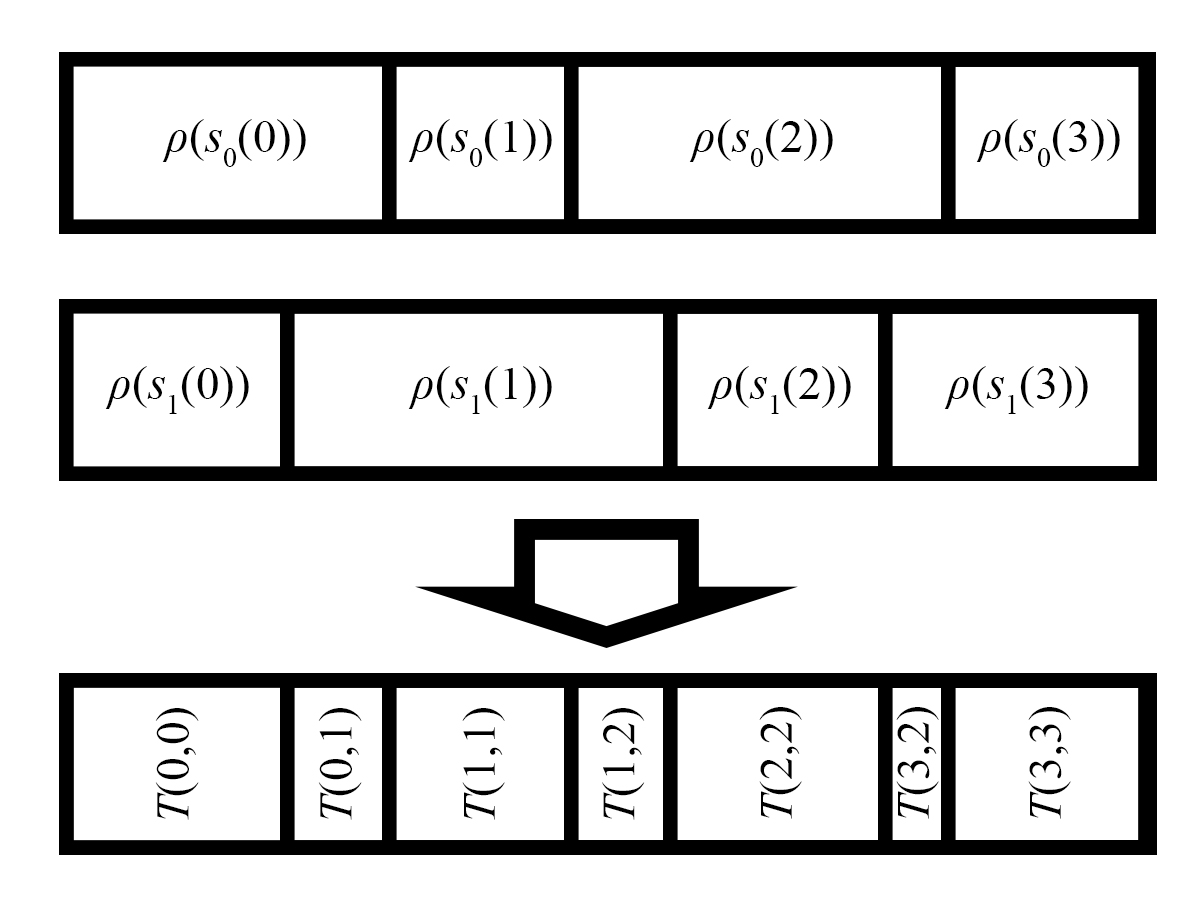
\includegraphics[width=0.7\textwidth]{figures/TransportDiagram}
  \caption{A visualization of the 1D optimal transport algorithm.
  The width of the bins represents the amount of mass in that bin.}
  \label{fig:optimaltransport}
\end{center}
\end{figure}

This algorithm runs linearly and guarantees that $T$ will be sparse with no more than $2N - 1$ entries.
This algorithm is visualized in figure~\ref{fig:optimaltransport}


%Using this algorithm, the number of assignments is $2N - 1$.

%From this point we could perform an interpolation.
%With interpolation factor $k$ the new peak index would be
%\begin{align}
  %c' = (1 - k)c(s_0) + k(c(s_1))
%\end{align}
%However we must first deal with the phase
\subsection{Phase Accumulation}

\begin{figure}[!h]
  %{r}{0.65\textwidth}
  \begin{center}
  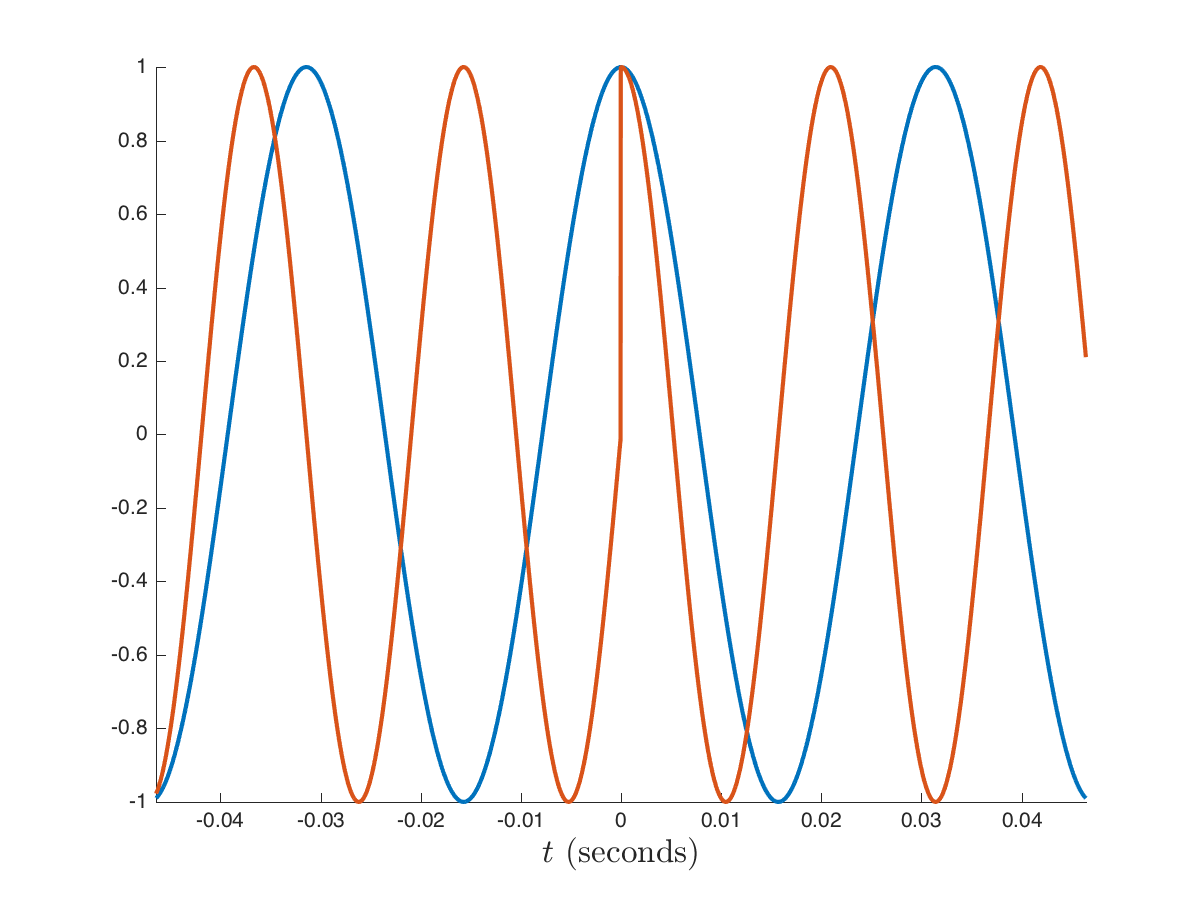
\includegraphics[width=0.7\textwidth]{figures/HorizontalIncoherence0}
  \caption{%
    The pitch of the original signal in blue is increased to be that of the orange signal.
  The window boundary at $t = 0$ experiences horizontal incoherence.}
  \label{fig:horizontalincoherence}
\end{center}
\end{figure}

After we have a transport map, we need to actually repitch the spectral segments.
When we move a segment of the spectrum to a new pitch, 
the phases within that section rotate either slower or faster.
This change does not make an audible difference within a window itself,
but it can cause interference in the overlap between windows known as \emph{horizontal incoherence} seen in figure~\ref{fig:horizontalincoherence}.

One solution to this in the realm of phase vocoders is to estimate the phase of the next frame based on its instantaneous frequency
\cite{vocoder}.
If a sinusoid with phase $\angle X(\omega, \tau)$ 
is oscillating with instantaneous frequency $\hat{\omega}(\omega)$ over frame $\tau$, we would expect the phase of the next frame to be
\begin{align}
  \angle X(\omega, \tau+1) = 
  \angle X(\omega,\tau) + \frac{R}{f_s}\hat{\omega}(\omega)
\end{align}
This model is good for signals which do not undergo rapid changes in frequency. 
However it does a poor job of dealing with transients in audio that can happen from sharp note attacks and percussive sounds. 
To cope with this, some phase vocoders employ phase reinitialization steps in frames where transients are detected.
Even with this step additional phasing can still occur
\cite{vocoder}.

Fortunately however, we have at our disposal the phases of not one but two pitches.
If we are interpolating along the transport map with interpolation factor $k$,
then for a particular assignment between $s_0$ and $s_1$
we know the center frequency of the mass will oscillate at frequency:
\begin{align}
  \hat{\omega}' = (1 - k)\hat{\omega}(c(s_0)) + \hat{\omega}(c(s_1))
\end{align}
The accumulated phases 
$\Theta_0(\omega, \tau)$
and
$\Theta_1(\omega, \tau)$
each change proportional to $\omega_0$
and $\omega_1$.
So to get a new phase $\Theta'$ whose rate of change is proportional to $\hat{\omega}'$, we can linearly interpolate between $\Theta_0$ and $\Theta_1$.
\begin{align}
  \Theta' = (1 - k)\Theta_0(\omega, \tau) + k\Theta_1(\omega, \tau)
\end{align}
We calculate the accumulated phase so that it increases with respect to $\hat{\omega}$, but round it to maintain the exact phase. This rounding is essentially a reinitialization every step, which we get away with because of the two sources.
\begin{align}
  \Theta(\omega, \tau) &\approx
  \sum_{t = 0}^\tau 
  \frac{R}{f_s}\hat{\omega}(\omega, \tau)\\
  \Theta(\omega, \tau) &= \Theta(\omega,\tau)\pmod{2\pi}
\end{align}

\subsection{Resynthesis}

\begin{algorithm}
  \caption{Resynthesize}\label{resynthesize}
\begin{algorithmic}
\\
\For{all $n$}
  \State{$Y(n) \leftarrow 0$}
  \Comment{Clear the output}
\EndFor
\\
\For{$i$, $j$}
  \\
  \State{$c' \leftarrow (1 - k)c(s_0(i)) + kc(s_1(j))$}
  \Comment{$c'$ is the new center index}
  \State{$\Theta' \leftarrow (1 - k)\Theta(c(s_0(i))) + k\Theta(c(s_1(j)))$}
  \Comment{$\Theta'$ is the new center phase}
  \\
  \For{$n\in U(s_0(i))$}
    \\
    \State{$n' \leftarrow n + \hat{n} - c(s_0(i))$}
    \Comment{$n'$ is the new bin index}
    \State{$\theta' \leftarrow \Theta_0(n) + \Theta' - \Theta_0(c(s_0(i)))$}
    \Comment{$\Theta'$ is the new bin phase}
    \\
    \State{%
      $Y(n') 
      \leftarrow 
      Y(n') +
      (1 - k)
      \frac{T(i, j)}{\rho(s_0(i))}
      |X_0(n)|
      e^{i\theta'}$
    }
    \Comment{Linearly interpolate}
    \\
  \EndFor

  \For{$n\in U(s_1(j))$}
    \\
    \State{$n' \leftarrow n + \hat{n} - c(s_1(j))$}
    \Comment{$n'$ is the new bin index}
    \State{$\theta' \leftarrow \Theta_1(n) + \Theta' - \Theta_1(c(s_1(j)))$}
    \Comment{$\Theta'$ is the new bin phase}
    \\
    \State{%
      $Y(n') 
      \leftarrow 
      Y(n') +
      j
      \frac{T(i, j)}{\rho(s_1(j))}
      |X_1(n)|
      e^{i\theta'}$
    }
    \Comment{Linearly interpolate}
    \\
  \EndFor
\EndFor
\end{algorithmic}
\end{algorithm}


After we have segmented, transported, and accumulated the phases, we can finally synthesize an output fourier transform $Y(n)$ as in algorithm~\ref{resynthesize}.
For every assignment, we find the new center frequency, and new center phase.
We then adjust all the phases within the segment to maintain local phase relations.
Finally we linearly interpolate between all of the segments according to the interpolation factor.

\section{Implementation}

I implemented the above algorithm in real-time as an audio effect in C++.
The program listens to two streams of audio
which can be sent to it from a any digital audio workstation.
It then produces a new stream of audio 
whose spectrum is transported between the two
according to a MIDI value.
The program depends on the library FFTW (Fastest Fourier Transform in the West) \cite{fftw} for Fourier transforms, and the open source libraries PortAudio\cite{portaudio} and PortMidi\cite{portmidi} for audio and MIDI handling respectively.

I work with a window size of 4096 samples and a sampling rate of 44,100 hertz.
This produces a delay of 10 milliseconds which is audible.
However the delay only exists on from the perspective of the source audio.
There is no perceivable delay from the perspective of the midi controller 
because the MIDI value is read right before a frame is synthesized.

Code: \href{https://github.com/sportdeath/Vocoder}{https://github.com/sportdeath/Vocoder}.

Video:
\href{https://youtu.be/PQGV0fk3Gww}{https://youtu.be/PQGV0fk3Gww}

\section{Conclusion}

As seen in the implementation video, the algorithm produces undistorted signals for a variety of inputs: monophonic - polyphonic, acoustic  - synthesized, bright - dark.

One of the most noticeable artifacts that still exists is the interference that results from a single pitch being mapped to many places.
As the note splits and moves to new locations it interferes with itself for the brief period of time where the splits overlap.
This artifact causes a drop in volume at the very start or end of a transport.
This type of interference has plagued music far before computers.
If adjacent semi-tones on a piano are played together you can hear beating.
As of now, I have no idea how to fix that other than performing a transport that
only maps a frequency to a single other frequency.
But that takes some of the fun away.
And in the end the distortion doesn't sound harsh and digital and in many cases the volume dip is barely noticeable.

Overall the effect produced a variety of interesting sounds.
This effect has potential both in the studio and live setting. It can be used by DJs to transition between songs or could be used by guitarists to swap between dualing solos.
It functions as a new way to filter between sounds of different timbres.
Moreover some of the sounds it produces sound simply unexplainable and I'm excited to explore their possibilities.

\nocite{*}
\bibliographystyle{plain}
\bibliography{bibliography}

\end{document}

Fundemental theory

that phase vocoder one

1d transport paper?

STFT

weighted overlap add

fftw

portaudio

portmidi

cite justin solomon




PLOT:
optimal transport
plot reassigned frequency
plot segmentation
plot buffered segmentation
plot misaligned audio
Phasing

Why did I do this frequency reassignment method?

It can pick peaks in the presence of noise, but no threshold so even small peaks can be detected.

Doesn't require setting a peak threshold 

Then Write algorithm for frequency

Clean up phase accumulation math

What are the symbols in resynthesize for center and phase

Then clean up some text

Then do references

Then do slides

Then do Demo

Get rid of optimal transport and phase vocoder sections
Put description of optimal transport in the introduction.
Intersperse Phase vocoder stuff
